\documentclass{article}\usepackage[]{graphicx}\usepackage[]{color}
% maxwidth is the original width if it is less than linewidth
% otherwise use linewidth (to make sure the graphics do not exceed the margin)
\makeatletter
\def\maxwidth{ %
  \ifdim\Gin@nat@width>\linewidth
    \linewidth
  \else
    \Gin@nat@width
  \fi
}
\makeatother

\definecolor{fgcolor}{rgb}{0.345, 0.345, 0.345}
\newcommand{\hlnum}[1]{\textcolor[rgb]{0.686,0.059,0.569}{#1}}%
\newcommand{\hlstr}[1]{\textcolor[rgb]{0.192,0.494,0.8}{#1}}%
\newcommand{\hlcom}[1]{\textcolor[rgb]{0.678,0.584,0.686}{\textit{#1}}}%
\newcommand{\hlopt}[1]{\textcolor[rgb]{0,0,0}{#1}}%
\newcommand{\hlstd}[1]{\textcolor[rgb]{0.345,0.345,0.345}{#1}}%
\newcommand{\hlkwa}[1]{\textcolor[rgb]{0.161,0.373,0.58}{\textbf{#1}}}%
\newcommand{\hlkwb}[1]{\textcolor[rgb]{0.69,0.353,0.396}{#1}}%
\newcommand{\hlkwc}[1]{\textcolor[rgb]{0.333,0.667,0.333}{#1}}%
\newcommand{\hlkwd}[1]{\textcolor[rgb]{0.737,0.353,0.396}{\textbf{#1}}}%
\let\hlipl\hlkwb

\usepackage{framed}
\makeatletter
\newenvironment{kframe}{%
 \def\at@end@of@kframe{}%
 \ifinner\ifhmode%
  \def\at@end@of@kframe{\end{minipage}}%
  \begin{minipage}{\columnwidth}%
 \fi\fi%
 \def\FrameCommand##1{\hskip\@totalleftmargin \hskip-\fboxsep
 \colorbox{shadecolor}{##1}\hskip-\fboxsep
     % There is no \\@totalrightmargin, so:
     \hskip-\linewidth \hskip-\@totalleftmargin \hskip\columnwidth}%
 \MakeFramed {\advance\hsize-\width
   \@totalleftmargin\z@ \linewidth\hsize
   \@setminipage}}%
 {\par\unskip\endMakeFramed%
 \at@end@of@kframe}
\makeatother

\definecolor{shadecolor}{rgb}{.97, .97, .97}
\definecolor{messagecolor}{rgb}{0, 0, 0}
\definecolor{warningcolor}{rgb}{1, 0, 1}
\definecolor{errorcolor}{rgb}{1, 0, 0}
\newenvironment{knitrout}{}{} % an empty environment to be redefined in TeX

\usepackage{alltt}

\usepackage{float}

% Set the margins on the page to not be so large
\addtolength{\oddsidemargin}{-.875in}
\addtolength{\evensidemargin}{-.875in}
\addtolength{\textwidth}{1.75in}
\addtolength{\topmargin}{-.875in}
\addtolength{\textheight}{1.75in}

% Take off page numbering
\pagenumbering{gobble}
\IfFileExists{upquote.sty}{\usepackage{upquote}}{}
\begin{document}

\title{%
  5.1.1 - R: Logistic Regression \\
  \smallskip
  \large Stat 5100: Dr. Bean
}
\date{}

\maketitle

\textbf{Example:} (Text Table 14.3)  Individuals were randomly sampled within two sectors of a city, and checked for presence of disease (here, spread by mosquitoes).  Subjects’ age (in years), socioeconomic status (low, medium, high), and city sector are to be used to predict the \underline{probability of contracting the disease.}

In R, we can create logistic regression models with the glm function. ``GLM'' stands for generalized linear model, and can be used to fit a variety of linear models. To specify logistic regression, we set an option in side the glm function that specifies a binomial (two classes) response.

\subsubsection*{Fit a logistic regression model}

\begin{knitrout}
\definecolor{shadecolor}{rgb}{0.969, 0.969, 0.969}\color{fgcolor}\begin{kframe}
\begin{alltt}
\hlcom{# Input the data}
\hlkwd{library}\hlstd{(stat5100)}
\hlkwd{data}\hlstd{(outbreak)}

\hlstd{outbreak_logreg} \hlkwb{<-} \hlkwd{glm}\hlstd{(disease} \hlopt{~} \hlstd{age} \hlopt{+} \hlstd{SES_mid} \hlopt{+} \hlstd{SES_low} \hlopt{+} \hlstd{sector,}
                       \hlkwc{data} \hlstd{= outbreak,} \hlkwc{family} \hlstd{=} \hlstr{"binomial"}\hlstd{)}
\hlkwd{summary}\hlstd{(outbreak_logreg)}
\end{alltt}
\begin{verbatim}
## 
## Call:
## glm(formula = disease ~ age + SES_mid + SES_low + sector, family = "binomial", 
##     data = outbreak)
## 
## Deviance Residuals: 
##     Min       1Q   Median       3Q      Max  
## -1.6552  -0.7529  -0.4788   0.8558   2.0977  
## 
## Coefficients:
##             Estimate Std. Error z value Pr(>|z|)    
## (Intercept) -2.31293    0.64259  -3.599 0.000319 ***
## age          0.02975    0.01350   2.203 0.027577 *  
## SES_mid1     0.40879    0.59900   0.682 0.494954    
## SES_low1    -0.30525    0.60413  -0.505 0.613362    
## sector1      1.57475    0.50162   3.139 0.001693 ** 
## ---
## Signif. codes:  0 '***' 0.001 '**' 0.01 '*' 0.05 '.' 0.1 ' ' 1
## 
## (Dispersion parameter for binomial family taken to be 1)
## 
##     Null deviance: 122.32  on 97  degrees of freedom
## Residual deviance: 101.05  on 93  degrees of freedom
## AIC: 111.05
## 
## Number of Fisher Scoring iterations: 4
\end{verbatim}
\end{kframe}
\end{knitrout}

\subsubsection*{Plot a graph of observed values and predicted probabilities}

Because we have multiple predictor variables, we have to choose one variable to put on the x-axis, and the rest of the variables will have to be fixed at some value. We will use Age for our x-axis variable. We will set SES_mid = 0.245, SES_low = 0.367, and Sector = 0.398.

\begin{knitrout}
\definecolor{shadecolor}{rgb}{0.969, 0.969, 0.969}\color{fgcolor}\begin{kframe}
\begin{alltt}
\hlcom{# Get a range of ages, and then predict the probability with the predict()}
\hlcom{# function to get the shape of the predicted probability curve.}
\hlstd{age_range} \hlkwb{<-} \hlkwd{seq}\hlstd{(}\hlnum{0}\hlstd{,} \hlnum{80}\hlstd{,} \hlkwc{length} \hlstd{=} \hlnum{500}\hlstd{)}
\hlstd{npred} \hlkwb{<-} \hlkwd{length}\hlstd{(age_range)}

\hlstd{pred_data} \hlkwb{<-} \hlkwd{data.frame}\hlstd{(}\hlkwc{age} \hlstd{= age_range,} \hlkwc{SES_mid} \hlstd{=} \hlkwd{as.factor}\hlstd{(}\hlkwd{rep}\hlstd{(}\hlnum{0.245}\hlstd{, npred)),}
                        \hlkwc{SES_low} \hlstd{=} \hlkwd{as.factor}\hlstd{(}\hlkwd{rep}\hlstd{(}\hlnum{0.367}\hlstd{, npred)),}
                        \hlkwc{sector} \hlstd{=} \hlkwd{as.factor}\hlstd{(}\hlkwd{rep}\hlstd{(}\hlnum{0.398}\hlstd{, npred)))}
\hlstd{pred_disease} \hlkwb{<-} \hlkwd{predict}\hlstd{(outbreak_logreg,} \hlkwc{newdata} \hlstd{= pred_data,} \hlkwc{type} \hlstd{=} \hlstr{"response"}\hlstd{)}
\end{alltt}


{\ttfamily\noindent\bfseries\color{errorcolor}{\#\# Error in model.frame.default(Terms, newdata, na.action = na.action, xlev = object\$xlevels): factor SES\_mid has new level 0.245}}\begin{alltt}
\hlkwd{plot}\hlstd{(outbreak}\hlopt{$}\hlstd{age,} \hlkwd{as.numeric}\hlstd{(outbreak}\hlopt{$}\hlstd{disease))}
\end{alltt}
\end{kframe}

{\centering 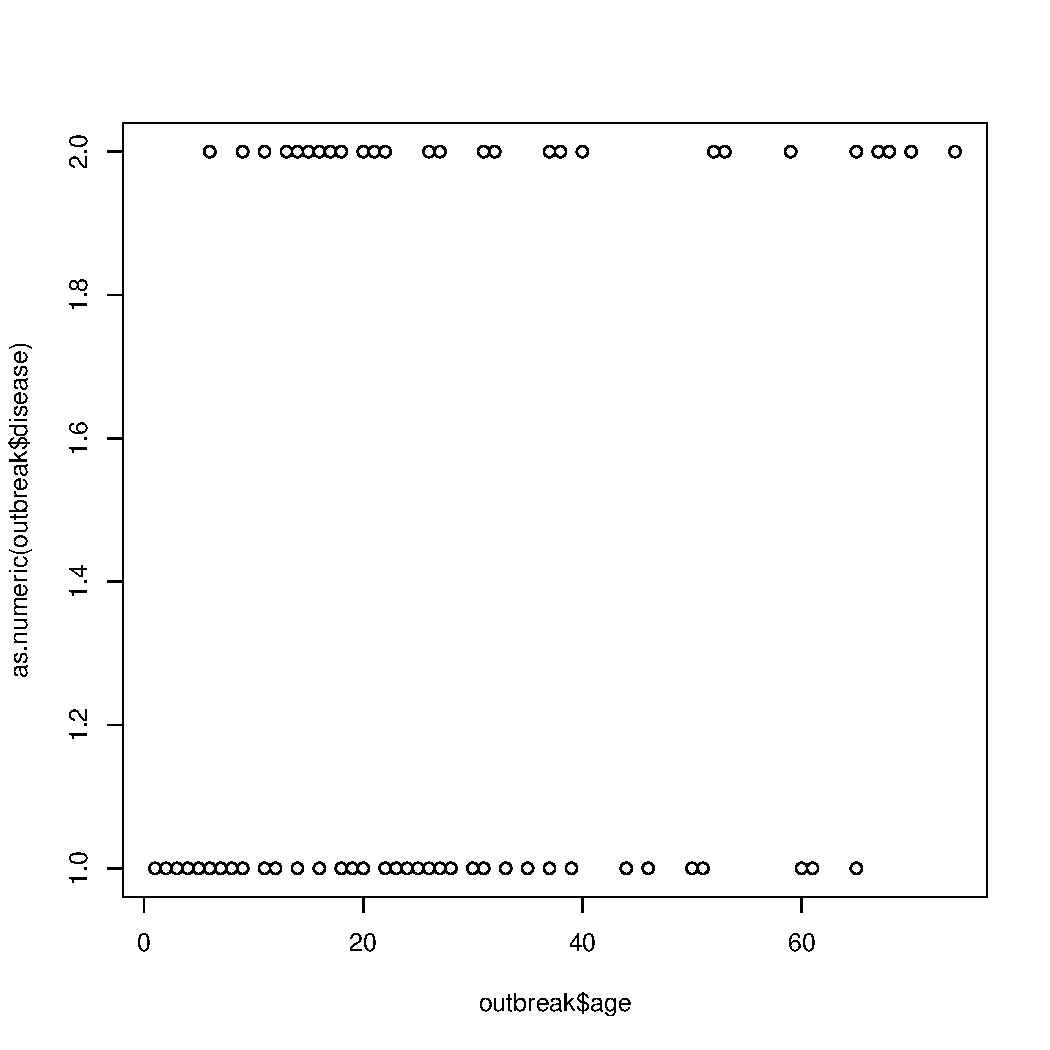
\includegraphics[width=0.6\textwidth]{figure/unnamed-chunk-2-1} 

}



\end{knitrout}

\begin{knitrout}
\definecolor{shadecolor}{rgb}{0.969, 0.969, 0.969}\color{fgcolor}\begin{kframe}
\begin{alltt}
\hlcom{# Input the data}
\hlkwd{library}\hlstd{(stat5100)}
\hlkwd{data}\hlstd{(outbreak)}

\hlstd{outbreak_logreg} \hlkwb{<-} \hlkwd{glm}\hlstd{(disease} \hlopt{~} \hlstd{age} \hlopt{+} \hlstd{SES_mid} \hlopt{+} \hlstd{SES_low} \hlopt{+} \hlstd{sector,}
                       \hlkwc{data} \hlstd{= outbreak,} \hlkwc{family} \hlstd{=} \hlstr{"binomial"}\hlstd{)}
\hlkwd{summary}\hlstd{(outbreak_logreg)}
\end{alltt}
\begin{verbatim}
## 
## Call:
## glm(formula = disease ~ age + SES_mid + SES_low + sector, family = "binomial", 
##     data = outbreak)
## 
## Deviance Residuals: 
##     Min       1Q   Median       3Q      Max  
## -1.6552  -0.7529  -0.4788   0.8558   2.0977  
## 
## Coefficients:
##             Estimate Std. Error z value Pr(>|z|)    
## (Intercept) -2.31293    0.64259  -3.599 0.000319 ***
## age          0.02975    0.01350   2.203 0.027577 *  
## SES_mid1     0.40879    0.59900   0.682 0.494954    
## SES_low1    -0.30525    0.60413  -0.505 0.613362    
## sector1      1.57475    0.50162   3.139 0.001693 ** 
## ---
## Signif. codes:  0 '***' 0.001 '**' 0.01 '*' 0.05 '.' 0.1 ' ' 1
## 
## (Dispersion parameter for binomial family taken to be 1)
## 
##     Null deviance: 122.32  on 97  degrees of freedom
## Residual deviance: 101.05  on 93  degrees of freedom
## AIC: 111.05
## 
## Number of Fisher Scoring iterations: 4
\end{verbatim}
\end{kframe}
\end{knitrout}

\begin{knitrout}
\definecolor{shadecolor}{rgb}{0.969, 0.969, 0.969}\color{fgcolor}\begin{kframe}
\begin{alltt}
\hlcom{# ROC Curve}
\hlstd{prob} \hlkwb{<-} \hlkwd{predict}\hlstd{(outbreak_logreg,} \hlkwc{newdata} \hlstd{= outbreak,} \hlkwc{type} \hlstd{=} \hlstr{"response"}\hlstd{)}
\hlstd{pROC}\hlopt{::}\hlkwd{roc}\hlstd{(outbreak}\hlopt{$}\hlstd{disease} \hlopt{~} \hlstd{prob,} \hlkwc{plot} \hlstd{=} \hlnum{TRUE}\hlstd{,} \hlkwc{print.auc} \hlstd{=} \hlnum{TRUE}\hlstd{)}
\end{alltt}


{\ttfamily\noindent\itshape\color{messagecolor}{\#\# Setting levels: control = 0, case = 1}}

{\ttfamily\noindent\itshape\color{messagecolor}{\#\# Setting direction: controls < cases}}\end{kframe}

{\centering 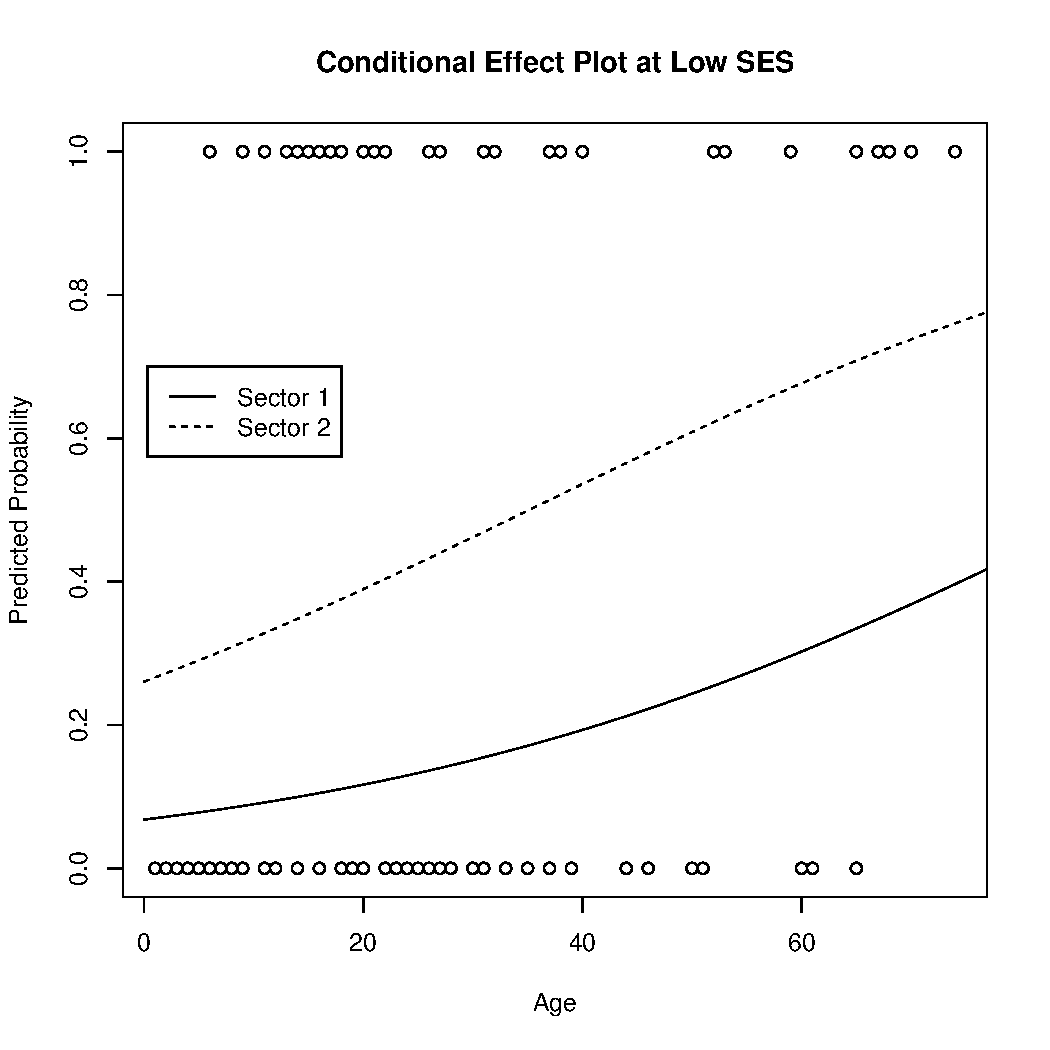
\includegraphics[width=0.6\textwidth]{figure/unnamed-chunk-4-1} 

}


\begin{kframe}\begin{verbatim}
## 
## Call:
## roc.formula(formula = outbreak$disease ~ prob, plot = TRUE, print.auc = TRUE)
## 
## Data: prob in 67 controls (outbreak$disease 0) < 31 cases (outbreak$disease 1).
## Area under the curve: 0.7764
\end{verbatim}
\end{kframe}
\end{knitrout}

\end{document}
